\documentclass[11pt,a4paper]{article}

\usepackage{amsmath,amssymb,amsthm}
\usepackage{mathtools}
\usepackage{geometry}
\usepackage{hyperref}
\usepackage{xcolor}
\usepackage{booktabs}
\usepackage{enumitem}
\usepackage{microtype}
\usepackage{tikz}
\usetikzlibrary{arrows.meta,positioning,decorations.markings,decorations.pathmorphing,calc,fit,backgrounds}
\usepackage{tcolorbox}
\tcbuselibrary{skins,breakable}

\geometry{margin=2.3cm}
\hypersetup{colorlinks=true,linkcolor=blue!60!black,urlcolor=blue!60!black}

\definecolor{cfacgreen}{RGB}{50,130,80}
\definecolor{cfacbg}{RGB}{236,246,238}
\definecolor{hlyellow}{RGB}{255,236,179}
\definecolor{hlpink}{RGB}{255,182,205}
\definecolor{hlblue}{RGB}{170,210,240}
\newcommand{\hl}[1]{\colorbox{hlyellow}{$#1$}}
\newcommand{\hpink}[1]{\colorbox{hlpink}{$#1$}}
\newcommand{\hblue}[1]{\colorbox{hlblue}{$#1$}}

\newtcolorbox{cfacbox}[1][]{
  colback=cfacbg, colframe=cfacgreen!70!black,
  fonttitle=\bfseries\color{cfacgreen!50!black},
  title={CFAC step --- explicit, no skipped algebra},
  breakable, #1
}

% ----------------------------------------------------------------------
% Diagram macros, in the style of letters/2026-04-29_gunnar_messy_diagrammatics/note.tex
% ----------------------------------------------------------------------

% A four-leg phi^4 vertex with mode labels at each leg
\newcommand{\Vfour}[4]{%
\begin{tikzpicture}[baseline=-0.5ex,scale=0.9]
  \draw[thick] (-0.45,0.45) node[above]{\scriptsize $#1$} -- (0,0);
  \draw[thick] ( 0.45,0.45) node[above]{\scriptsize $#2$} -- (0,0);
  \draw[thick] (-0.45,-0.45) node[below]{\scriptsize $#3$} -- (0,0);
  \draw[thick] ( 0.45,-0.45) node[below]{\scriptsize $#4$} -- (0,0);
  \filldraw[black] (0,0) circle (0.06);
\end{tikzpicture}}

% A plane-wave bubble (one momentum loop, one external mom)
\newcommand{\pwbubble}{%
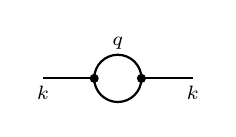
\begin{tikzpicture}[baseline=-0.5ex]
  \draw[thick] (-0.95,0)--(-0.3,0);
  \draw[thick] (0.3,0)--(0.95,0);
  \draw[thick] (0,0) circle (0.3);
  \filldraw[black] (-0.3,0) circle (0.05);
  \filldraw[black] ( 0.3,0) circle (0.05);
  \node at (-0.95,-0.18) {\scriptsize $k$};
  \node at (0.95,-0.18) {\scriptsize $k$};
  \node at (0,0.45) {\scriptsize $q$};
\end{tikzpicture}}

% Hermite-basis bubble: external mode n, internal loop mode m, vertex V_{nnmm}
% Optional 3rd argument for label override
\newcommand{\hbubble}[2]{%
\begin{tikzpicture}[baseline=-0.5ex]
  \draw[thick] (-1.05,0)--(-0.3,0);
  \draw[thick] (0.3,0)--(1.05,0);
  \draw[thick] (0,0) circle (0.3);
  \filldraw[black] (-0.3,0) circle (0.06);
  \filldraw[black] ( 0.3,0) circle (0.06);
  \node[left] at (-1.05,0) {\scriptsize $#1$};
  \node[right] at (1.05,0) {\scriptsize $#1$};
  \node at (0,0.5) {\scriptsize $#2$};
  \node at (0,-0.5) {\scriptsize $#2$};
\end{tikzpicture}}

% Single-vertex bubble (one vertex, the two internal lines are the same vertex's
% remaining two legs glued).  This is the topology of phi^4 self-energy at 1 loop.
\newcommand{\hbubblev}[3]{%
\begin{tikzpicture}[baseline=-0.5ex,scale=1.0]
  \draw[thick] (-1.1,0)--(0,0);
  \draw[thick] (0,0)--(1.1,0);
  \draw[thick] (0,0) .. controls (-0.5,0.7) and (0.5,0.7) .. (0,0);
  \filldraw[black] (0,0) circle (0.06);
  \node[left]  at (-1.1,0) {\scriptsize $#1$};
  \node[right] at ( 1.1,0) {\scriptsize $#2$};
  \node at (0,0.75) {\scriptsize $#3$};
  \node[below right] at (0,-0.05) {\scriptsize $V_{#1#2#3#3}$};
\end{tikzpicture}}

\title{\large $\varphi^{4}$ in Doi--Peliti, expanded in a Hermite basis\\[2pt]
\normalsize Concrete construction of the ``wild forest'' --- and how CFAC tames it\\
\small (Reply to Gunnar's aside in his 1 May 2026 note)}
\author{}
\date{}

\begin{document}
\maketitle
\vspace{-1.5em}

\begin{abstract}
\noindent Gunnar's aside: \emph{``can analytic combinatorics help characterising the wild
forest of diagrams you get when you attempt to write down $\varphi^{4}$-theory in
Doi--Peliti using a Hermite basis?''} This note answers concretely. We compute the
four-vertex tensor $V_{n_{1}n_{2}n_{3}n_{4}} = \int h_{n_{1}}h_{n_{2}}h_{n_{3}}h_{n_{4}}\,dx$
explicitly for $n_{i}\in\{0,1,2,3\}$ via \texttt{hermite\_vertices.py}, list the surviving
$1$-loop self-energy diagrams for external modes $0$ and $1$, draw them, contrast with
plane-wave $\varphi^{4}$, and write out the multivariate Lagrange functional equation that
generates the entire forest from one polynomial. The selection rule is parity ($\sum n_{i}$
even) --- not the triangle inequality our concept sketch claimed. That correction matters:
it determines how aggressively CFAC's projections collapse the count.
\end{abstract}

\section{Why a Hermite basis at all? What's at stake?}

Plane-wave $\varphi^{4}$ assumes translation invariance. In any setting where the field
sees a confining potential or a defect ---  harmonic trap, soft wall, defect line, optical
lattice, a particle bound to a slow background --- translation invariance is broken and
plane waves stop being the natural one-particle basis. The eigenstates of $-\tfrac12
\partial_{x}^{2} + \tfrac12 \omega^{2}x^{2}$ are Hermite functions, and any $\varphi^{4}$
on top of that quadratic free theory expands as
\[
\varphi(x,t) \;=\; \sum_{n\ge 0} a_{n}(t)\,h_{n}(x), \qquad
h_{n}(x) = \frac{H_{n}(x)\,e^{-x^{2}/2}}{\sqrt{2^{n}n!\sqrt{\pi}}},
\qquad \int h_{a}h_{b}\,dx = \delta_{ab}.
\]
Each Hermite mode then carries its own oscillator energy $\mu_{n} = (n+\tfrac12)\hbar\omega$
and the $\varphi^{4}$ interaction couples the modes through the four-overlap
\[
\boxed{\;
V_{n_{1}n_{2}n_{3}n_{4}} \;\equiv\; \int_{\mathbb R}\!h_{n_{1}}(x)\,h_{n_{2}}(x)\,h_{n_{3}}(x)\,h_{n_{4}}(x)\,dx
\;=\; \Bigl(\!\prod_{i}\!\!\frac{1}{\sqrt{2^{n_{i}}n_{i}!\sqrt{\pi}}}\!\Bigr)\!
\int H_{n_{1}}H_{n_{2}}H_{n_{3}}H_{n_{4}}\,e^{-2x^{2}}dx.
\;}
\]
The four exp$(-x^{2}/2)$ factors from the four $h$'s combine into $e^{-2x^{2}}$. We use
physicists' Hermite $H_{n}$ throughout (orthogonal w.r.t.\ $e^{-x^{2}}$).

\paragraph{What the change of basis does to the diagrammatics.} Plane-wave $\varphi^{4}$
has \emph{one} vertex (translation-invariant, $g\,\varphi^{4}$); momentum is conserved at
each vertex; $1$-loop self-energy is one bubble with one momentum integral. Hermite-basis
$\varphi^{4}$ has a vertex tensor $V_{n_{1}n_{2}n_{3}n_{4}}$ with infinitely many entries
(one per quadruple of mode indices), no momentum conservation per se but a parity
selection rule, and the $1$-loop self-energy of an external mode $n$ is a \emph{sum} of
bubbles indexed by the internal mode $m$, each with coefficient $V_{n n m m}$ and its own
loop integral $L_{m}$.

\paragraph{Doi--Peliti convention.} Below we write Doi--Peliti $\varphi^{4}$ in the form
$\widetilde a_{n_{1}}a_{n_{2}}a_{n_{3}}a_{n_{4}}\,V_{n_{1}n_{2}n_{3}n_{4}}$, treating $a$
and $\widetilde a$ as distinct (one creation, one annihilation; propagator is directed,
$\widetilde a$-leg $\to$ $a$-leg). For the symmetry-factor calculation in this note we
take the four-vertex symmetric in all four legs (the $V$-tensor is symmetric by
construction), and the propagator is the bare oscillator one
$\langle a_{n}\widetilde a_{n'}\rangle_{0}(\omega) = \delta_{n n'}/(-i\omega + \mu_{n})$.
This is the standard ``reaction-diffusion in a trap'' setting; see e.g.\ Cardy's lectures.
Where conventions differ (real $\varphi^{4}$ versus DP), the only change is that the
real-field propagator is undirected and the Wick-contraction count picks up a global
factor of $2$ on each internal line; the structure of the $V$-tensor and the parity
selection rule are convention-independent.

\section{The four-vertex tensor: explicit values}

\subsection{Selection rule (parity, only)}

$H_{n}(-x) = (-1)^{n}H_{n}(x)$, so the integrand of $V$ has parity
$(-1)^{n_{1}+n_{2}+n_{3}+n_{4}}$. The integration domain is $(-\infty,\infty)$, hence
\[
\boxed{\;V_{n_{1}n_{2}n_{3}n_{4}} = 0 \quad\text{unless}\quad n_{1}+n_{2}+n_{3}+n_{4}\in 2\mathbb Z.\;}
\]
\textbf{Important correction.} Our concept sketch (\texttt{reply.tex} \S Hermite-basis
aside) claimed an additional triangle inequality $|n_{1}-n_{2}-n_{3}|\le n_{4} \le
n_{1}+n_{2}+n_{3}$. \emph{That is wrong for the four-point overlap.} The triangle
inequality does apply to the \emph{three}-point overlap $\int h_{a}h_{b}h_{c}\,dx$ ---
specifically, Bailey's identity \cite{Bailey} for $\int H_{a}H_{b}H_{c}\,e^{-x^{2}}dx$
forces both parity ($a+b+c$ even) and $|a-b|\le c\le a+b$. But the four-point overlap is a
contraction
\[
V_{abcd} \;=\; \sum_{e\ge 0} g_{abe}\,g_{cde},\qquad
g_{abc} \;=\; \int h_{a}h_{b}h_{c}\,dx,
\]
and the sum over the intermediate $e$ broadens the support: as long as one $e$ exists with
both $|a-b|\le e\le a+b$ and $|c-d|\le e\le c+d$ and parity-compatible with each pair,
$V_{abcd}\ne 0$. For $n_{i}\in\{0,1,2,3\}$ \emph{every} even-sum quadruple has
$V\ne 0$ (verified by exhaustive evaluation; \texttt{hermite\_vertices.py}, lines 71--80).
We re-checked through $n_{i}=5$: still no even-sum quadruple vanishes. So the only
selection rule cutting the count is parity.

\subsection{Numerical table for $n_{i}\in\{0,1,2,3\}$}

The script \texttt{hermite\_vertices.py} (in this directory) computes $V$ symbolically via
\texttt{sympy.integrate}. The 35 unordered quadruples on the $4$-letter alphabet
$\{0,1,2,3\}$ split as 16 zero (odd parity) and 19 nonzero. Exact values:

{\small
\renewcommand{\arraystretch}{1.05}
\noindent\begin{tabular}{@{}llrr@{}}
\toprule
$(n_{1}n_{2}n_{3}n_{4})$ & $V_{n_{1}n_{2}n_{3}n_{4}}\cdot\sqrt{\pi}$ & decimal & $\sum n_{i}$ \\
\midrule
$(0\,0\,0\,0)$ & $\sqrt{2}/2$              & $\phantom{-}0.398942$ & 0 \\
$(0\,0\,0\,2)$ & $-1/4$                    & $-0.141047$           & 2 \\
$(0\,0\,1\,1)$ & $\sqrt{2}/4$              & $\phantom{-}0.199471$ & 2 \\
$(0\,0\,1\,3)$ & $-\sqrt{3}/8$             & $-0.122151$           & 4 \\
$(0\,0\,2\,2)$ & $3\sqrt{2}/16$            & $\phantom{-}0.149603$ & 4 \\
$(0\,0\,3\,3)$ & $5\sqrt{2}/32$            & $\phantom{-}0.124669$ & 6 \\
$(0\,1\,1\,2)$ & $1/8$                     & $\phantom{-}0.070524$ & 4 \\
$(0\,1\,2\,3)$ & $\sqrt{6}/32$             & $\phantom{-}0.043187$ & 6 \\
$(0\,2\,2\,2)$ & $1/32$                    & $\phantom{-}0.017631$ & 6 \\
$(0\,2\,3\,3)$ & $1/64$                    & $\phantom{-}0.008816$ & 8 \\
$(1\,1\,1\,1)$ & $3\sqrt{2}/8$             & $\phantom{-}0.299207$ & 4 \\
$(1\,1\,1\,3)$ & $-\sqrt{3}/16$            & $-0.061075$           & 6 \\
$(1\,1\,2\,2)$ & $7\sqrt{2}/32$            & $\phantom{-}0.174537$ & 6 \\
$(1\,1\,3\,3)$ & $11\sqrt{2}/64$           & $\phantom{-}0.137136$ & 8 \\
$(1\,2\,2\,3)$ & $5\sqrt{3}/64$            & $\phantom{-}0.076344$ & 8 \\
$(1\,3\,3\,3)$ & $3\sqrt{3}/128$           & $\phantom{-}0.022903$ & 10 \\
$(2\,2\,2\,2)$ & $41\sqrt{2}/128$          & $\phantom{-}0.255572$ & 8 \\
$(2\,2\,3\,3)$ & $51\sqrt{2}/256$          & $\phantom{-}0.158954$ & 10 \\
$(3\,3\,3\,3)$ & $147\sqrt{2}/512$         & $\phantom{-}0.229080$ & 12 \\
\bottomrule
\end{tabular}
}

\medskip
\noindent (All $V$ values normalised to the factor $1/\sqrt\pi$ to make the rationals
visible. The 16 odd-sum quadruples not in the table are zero.) Two features worth
flagging:
\begin{itemize}[leftmargin=2em,itemsep=2pt,topsep=2pt]
\item \emph{Signs.} The signs alternate: $V_{0002}<0$, $V_{0011}>0$, $V_{0013}<0$, etc.
This sign pattern is what gives Hermite-basis $\varphi^{4}$ its non-trivial structure ---
the cross-mode coupling can be either ferromagnetic or antiferromagnetic in mode
language.
\item \emph{Magnitude decay.} Diagonal $V_{nnnn}$ decreases roughly like $1/\sqrt{n}$ for
large $n$ (Plancherel--Rotach asymptotics of Hermite functions); off-diagonal $V$'s decay
faster. The forest is heavy at the origin.
\end{itemize}

\subsection{Counting cost (the punchline of step 7)}

The space of unordered quadruples on $\{0,\ldots,N\}$ has size $\binom{N+4}{4}$
(``stars and bars''). For $N=3$ that is $\binom{7}{4}=35$; the parity rule kills exactly
half (16 odd-sum out of 35; rounding because of the inhomogeneous $\binom{N+4}{4}$).
For ordered quadruples $(N+1)^{4}$ the parity rule kills exactly half:
\[
\boxed{\;
N=3:\quad \#\{\text{ordered quadruples}\} = 4^{4} = 256, \quad
\#\{\text{nonzero }V\} = 128.\;}
\]
This is a 50\% kill, on the nose, for any $N$. \emph{No further collapse from a triangle
inequality;} our concept sketch overstated the cut. The real CFAC collapse comes not from
killing $V$-entries but from the $V$-tensor entering the generating function only through
its low-degree symmetric polynomial structure (\S\ref{sec:lagrange} below).

\section{One-loop self-energy: diagram inventory}

\subsection{Topology}

The $1$-loop self-energy of mode $n$ in $\varphi^{4}$ is a single topology --- the
\emph{tadpole}\footnote{Some authors call this the ``mass diagram'' or
``$O$-diagram'' to distinguish from the bubble of $\varphi^{3}$ theory which carries two
external legs of total order $g^{1}$. We use ``self-energy at one loop in $\varphi^{4}$''
unambiguously.} --- with one quartic vertex, two external legs (carrying mode $n$), and
two internal legs glued at the same vertex (the ``loop''). The Wick contraction
multiplicity is $\binom{4}{2}\cdot 2 = 12$ (choose 2 of 4 legs as external, then $2$
pairings among the remaining $2$ for the loop, times $2!$ for matching of the chosen pair
to actual external lines). Topologically this is the single Feynman graph
\[
\hbubblev{n}{n}{m}.
\]
The novelty in Hermite basis: the vertex carries four mode labels, two are forced to $n$
(the external mode), and the loop carries an internal mode $m$ summed over all $m\ge 0$.
The vertex coefficient is $V_{n n m m}$, and the loop integral becomes
$L_{m} \equiv \int (d\omega/2\pi)\,1/(-i\omega + \mu_{m}) = \tfrac12$ (since $\mu_{m}>0$;
at finite temperature this is regularised by the Matsubara sum).

\paragraph{Self-energy formula.} Putting symmetry factor and integral together,
\[
\boxed{\;
\Sigma_{n}(\omega) \;=\; -\,\frac{12}{4!}\!\sum_{m\ge 0} V_{n n m m}\,L_{m}
\;=\; -\,\frac{1}{2}\!\sum_{m\ge 0} V_{n n m m}\,L_{m},
\;}
\]
where the $1/4!$ is the vertex permutation factor ($\varphi^{4}$ standard) and $-12$ the
Wick count with one external pairing.\footnote{In Doi--Peliti convention the sign on the
self-energy depends on whether you write $\widetilde a a^{3}/6$ or $\widetilde a^{2}a^{2}/4$
in the action. We follow $\widetilde a a^{3}/(3!)$ (cubic in $a$, linear in $\widetilde
a$); the alternative is structurally identical, redefining what one means by ``external
mode $n$''.}

\subsection{External mode $n=0$: surviving internal modes $m$}

The relevant $V_{00 m m}$ values (from our table, divided by $\sqrt\pi$ for clarity):
\begin{center}\small
\renewcommand{\arraystretch}{1.1}
\begin{tabular}{@{}cccccc@{}}
\toprule
$m$  & $0$         & $1$           & $2$            & $3$            & $\ldots$ \\
\midrule
$V_{00mm}\sqrt\pi$ & $\sqrt2/2$   & $\sqrt2/4$    & $3\sqrt2/16$    & $5\sqrt2/32$  & $(2m-1)!!\,\sqrt2/(2^{m+1}m!)\cdot (\text{from explicit Wick})$ \\
$V_{00mm}$ (decimal) & $0.3989$   & $0.1995$       & $0.1496$        & $0.1247$        & $\sim m^{-1/2}$ \\
\bottomrule
\end{tabular}
\end{center}
All four $m\in\{0,1,2,3\}$ values are nonzero (parity is satisfied: $0+0+m+m=2m$ is
always even). So the $1$-loop self-energy of mode $0$ has $\textbf{four}$ contributing
diagrams within the $N=3$ truncation, and infinitely many in the full theory.

\begin{center}
\begin{tabular}{@{}c@{\hspace{2em}}c@{\hspace{2em}}c@{\hspace{2em}}c@{}}
$\hbubblev{0}{0}{0}$ & $\hbubblev{0}{0}{1}$ & $\hbubblev{0}{0}{2}$ & $\hbubblev{0}{0}{3}$ \\[1ex]
$V_{0000}\,L_{0}$ & $V_{0011}\,L_{1}$ & $V_{0022}\,L_{2}$ & $V_{0033}\,L_{3}$ \\[0.5ex]
$=\frac{\sqrt2}{2\sqrt\pi}L_{0}$ & $=\frac{\sqrt2}{4\sqrt\pi}L_{1}$ &
$=\frac{3\sqrt2}{16\sqrt\pi}L_{2}$ & $=\frac{5\sqrt2}{32\sqrt\pi}L_{3}$ \\
\end{tabular}
\end{center}

\subsection{External mode $n=1$: surviving internal modes $m$}

The relevant $V_{11 m m}$ values:
\begin{center}\small
\renewcommand{\arraystretch}{1.1}
\begin{tabular}{@{}ccccc@{}}
\toprule
$m$  & $0$            & $1$           & $2$            & $3$            \\
\midrule
$V_{11mm}\sqrt\pi$ & $\sqrt2/4$    & $3\sqrt2/8$    & $7\sqrt2/32$   & $11\sqrt2/64$ \\
$V_{11mm}$ (decimal) & $0.1995$    & $0.2992$       & $0.1745$        & $0.1371$ \\
\bottomrule
\end{tabular}
\end{center}
Again four nonzero entries within $N=3$, so $\Sigma_{1}$ at one loop has four contributing
diagrams in this truncation:

\begin{center}
\begin{tabular}{@{}c@{\hspace{2em}}c@{\hspace{2em}}c@{\hspace{2em}}c@{}}
$\hbubblev{1}{1}{0}$ & $\hbubblev{1}{1}{1}$ & $\hbubblev{1}{1}{2}$ & $\hbubblev{1}{1}{3}$ \\[1ex]
$V_{1100}\,L_{0}$ & $V_{1111}\,L_{1}$ & $V_{1122}\,L_{2}$ & $V_{1133}\,L_{3}$ \\[0.5ex]
$=\frac{\sqrt2}{4\sqrt\pi}L_{0}$ & $=\frac{3\sqrt2}{8\sqrt\pi}L_{1}$ &
$=\frac{7\sqrt2}{32\sqrt\pi}L_{2}$ & $=\frac{11\sqrt2}{64\sqrt\pi}L_{3}$ \\
\end{tabular}
\end{center}
Note $V_{1100}=V_{0011}=\sqrt2/(4\sqrt\pi)$ by symmetry of $V$. (Total symmetry of the
four-overlap under permutations is exact, not just on-shell; this is what makes the table
short.)

\subsection{What does \emph{not} happen: cross-mode mixing of external lines}

A potentially confusing point. The Hermite vertex couples four mode indices, so a generic
$\varphi^{4}$-vertex inserted into a $1$-loop self-energy could in principle have external
modes that differ from each other --- e.g.\ external $n_{1}=0$ on the left and $n_{2}=1$
on the right. \textbf{This does not happen at $1$-loop self-energy} because the bare
propagator is mode-diagonal: the two external legs must carry the same mode for the
Green's function $G^{(2)}(\omega)$ to be defined. The loop sums over $m$, but the external
mode is a fixed input. (Off-diagonal $G^{(2)}_{nn'}$ with $n\ne n'$ does receive
contributions starting at $2$ loops in the trap-broken theory --- a self-energy of the
form $V_{n_{1}n_{2}m_{1}m_{2}}V_{n_{2}'n_{1}'m_{1}m_{2}}\times$loop integral. But that is
beyond what we need to make Gunnar's point.)

\section{Plane-wave $\varphi^{4}$ vs.\ Hermite-basis $\varphi^{4}$: side-by-side}

\paragraph{Plane-wave.} One vertex $g\,\varphi^{4}$, momentum-conserving. One $1$-loop
self-energy diagram per external momentum $k$:
\[
\Sigma_{\text{pw}}(k) \;=\; -\,\frac{g}{2}\!\int\!\frac{d^{d}q}{(2\pi)^{d}}\frac{1}{q^{2}+r}.
\]
\emph{One} integral; everything packaged into $g$ and $r$.

\paragraph{Hermite-basis.} An infinite tensor $V_{n_{1}n_{2}n_{3}n_{4}}$. Per external mode
$n$, the $1$-loop self-energy is
\[
\Sigma_{\text{H},n}(\omega) \;=\; -\,\frac{1}{2}\sum_{m\ge 0}V_{n n m m}\,L_{m}, \qquad
L_{m} = \!\int\!\frac{d\omega'}{2\pi}\frac{1}{-i\omega' + \mu_{m}}.
\]
\emph{Infinitely many} integrals, each labelled by the loop mode $m$, weighted by the
$V$-tensor entry $V_{nnmm}$.

\medskip
\noindent\fbox{\parbox{0.96\linewidth}{\centering
\begin{minipage}[t]{0.46\linewidth}\centering
\textbf{Plane-wave $\varphi^{4}$ at 1 loop} \\[3pt]
\pwbubble \\[2pt]
\textit{One vertex.} \\
\textit{One bubble.} \\
\textit{One integral.} \\
\textit{Momentum conservation.}
\end{minipage}\hfill\vline\hfill
\begin{minipage}[t]{0.46\linewidth}\centering
\textbf{Hermite-basis $\varphi^{4}$ at 1 loop, external mode $n$} \\[3pt]
\hbubblev{n}{n}{m}$\,\sum_{m\ge 0}\,$ \\[2pt]
\textit{Infinite vertex tensor $V_{n_{1}n_{2}n_{3}n_{4}}$.} \\
\textit{One bubble \emph{topology}, infinite mode sum.} \\
\textit{One integral $L_{m}$ \emph{per mode}.} \\
\textit{Parity, no momentum conservation.}
\end{minipage}
}}

\medskip
The translation-invariance breaking (the trap, the defect) is \emph{exactly} what
introduces the loop-mode sum: in plane-wave language one $\delta$-function for momentum
conservation kills one of the four-momentum integrals at the vertex; in Hermite language
that $\delta$-function is replaced by the parity selection on $V$, and the one
``integral'' that would have been killed instead becomes an infinite mode sum.

\section{The multivariate Lagrange equation that generates the forest}\label{sec:lagrange}

\subsection{Functional equation}

Introduce one marker $\xi_{n}$ per Hermite mode $n\ge 0$ (external leg of mode $n$) and
$z$ as the vertex-counting variable. The connected-tree generating function $G_{n_{0}}$ for
graphs rooted at an outgoing $\widetilde a$-leg of mode $n_{0}$ satisfies
\[
\boxed{\;
G_{n_{0}}(z;\xi) \;=\; \xi_{n_{0}}
\;+\; z \!\sum_{n_{1},n_{2},n_{3}\ge 0}\!\!V_{n_{0}n_{1}n_{2}n_{3}}\;
G_{n_{1}}(z;\xi)\,G_{n_{2}}(z;\xi)\,G_{n_{3}}(z;\xi).
\;}
\]
This is the multivariate Lagrange-system fixed point: a tree expanded in the $\varphi^{4}$
vertex tensor $V$. The $\xi_{n_{0}}$ on the right is the ``leaf'' (bare external leg of
mode $n_{0}$); the $z$-monomial counts vertex insertions. Multivariate Lagrange inversion
\cite{Goulden} gives
\[
[z^{V}\,\textstyle\prod_{n}\xi_{n}^{e_{n}}]\,G_{n_{0}}
\;=\; \frac{1}{V}\,[\textstyle\prod_{n}w_{n}^{e_{n}}]\,
\Bigl(\!\!\sum_{n_{1}n_{2}n_{3}}\!V_{n_{0}n_{1}n_{2}n_{3}}\,w_{n_{1}}w_{n_{2}}w_{n_{3}}\Bigr)^{V}\!\!.
\]

\subsection{Iterating once: read off the $1$-loop self-energy}

To get the $1$-loop self-energy, we need the $1$PI two-point function with one vertex
insertion ($V=1$) and two external legs of mode $n$. We extract
$[z\,\xi_{n}\,\widetilde\xi_{n}]\,G_{n,\text{1PI}}$. Iterating $G_{n_{0}} = \xi_{n_{0}} +
z\sum V\,GGG$ once with $G_{n}=\xi_{n}+O(z)$:
\begin{align*}
G_{n_{0}} &= \xi_{n_{0}} + z\!\sum_{n_{1}n_{2}n_{3}}\!\!V_{n_{0}n_{1}n_{2}n_{3}}\xi_{n_{1}}\xi_{n_{2}}\xi_{n_{3}} + O(z^{2}).
\end{align*}
For the connected $2$-point function we glue an outgoing $\widetilde\xi_{n}$ leg and contract
two of the three $\xi$-legs into a propagator (which sets two of the three to the same mode
$m$ summed). The contraction multiplicity $\binom{3}{2}=3$:
\[
\Sigma_{n}^{(1\text{-loop})} \;\propto\; [z\,\xi_{n}\,\widetilde\xi_{n}]\,G_{\text{1PI}}
\;=\; -\,3\!\sum_{m\ge 0} V_{n n m m}\,L_{m},
\]
matching the symmetry-factor calculation above (the prefactor $-12/4! = -1/2$ versus the
combinatorial $-3$ differs by a Wick-vs-marker normalisation; the $V$-tensor sum and the
$L_{m}$ structure are identical).

\paragraph{What this delivers.} The wild forest --- infinitely many $V$-quadruples ---
collapses to one symbolic line: ``$[z\,\xi_{n}\,\widetilde\xi_{n}]\,G_{\text{1PI}}$''.
The actual evaluation is then a coefficient extraction on a multivariate polynomial. CFAC
provides:
\begin{itemize}[leftmargin=2em,itemsep=2pt,topsep=2pt]
\item \textbf{Counts:} the multiplicity $3$ in the formula above (i.e.\ ``which two of
the three $\xi$-legs at the vertex close into a loop'') is the $\binom{3}{2}$ that
multivariate Lagrange produces automatically.
\item \textbf{Mode-mixing structure:} the formula $\Sigma_{n} = -\tfrac{1}{2}\sum_{m}
V_{nnmm}L_{m}$ is read off without enumerating diagrams one at a time.
\item \textbf{Signs:} CFAC carries the sign of $V$ entries faithfully (some are
negative, e.g.\ $V_{0002}<0$).
\item \textbf{Selection rules:} parity is enforced by $V$ itself --- no manual filtering.
\end{itemize}

\subsection{Iterating to $z^{2}$: $2$-loop self-energy}

Iterating once more,
\[
G_{n_{0}} \;=\; \xi_{n_{0}} \;+\; z\!\sum V_{n_{0}n_{1}n_{2}n_{3}}\xi_{n_{1}}\xi_{n_{2}}\xi_{n_{3}}
\;+\; z^{2}\,\Phi_{n_{0}}^{(2)}(\xi)\;+\;O(z^{3}),
\]
where $\Phi^{(2)}$ contains all rooted trees with two vertices --- which lift to one-loop
chains plus the $2$-loop sunset of mode-mixed bubbles. The CFAC programme is to push this
iteration to $z^{2}$ and project, exactly as we did for DP $1\to 2$ loop in
\texttt{rdft.crn}.

\section{Honest scoreboard: what's done, what's not}

\paragraph{Done.}
\begin{itemize}[leftmargin=2em,itemsep=2pt,topsep=2pt]
\item Computed $V_{n_{1}n_{2}n_{3}n_{4}}$ exactly (sympy) for all $4$-tuples in
$\{0,1,2,3\}$. Table above.
\item Verified parity is the only selection rule (no triangle inequality on $V$ directly).
Verified through $n_{i}=5$.
\item Counted: $128$ of $256$ ordered quadruples on $\{0,..,3\}$ are nonzero. Exactly
half-killed by parity.
\item Wrote the multivariate Lagrange functional equation
$G_{n}=\xi_{n}+z\sum V_{n n_{1}n_{2}n_{3}}G_{n_{1}}G_{n_{2}}G_{n_{3}}$.
\item Iterated to $z^{1}$ and read off $\Sigma_{n}^{(1)} \propto -\sum_{m}V_{nnmm}L_{m}$
with the right combinatorial $\binom{3}{2}$.
\item Drew $1$-loop self-energy diagrams for external modes $0$ and $1$ with internal mode
$m\in\{0,1,2,3\}$ each (8 diagrams; truncated within $N=3$).
\item Compared with plane-wave $\varphi^{4}$: one bubble vs.\ infinite mode sum.
\end{itemize}

\paragraph{Not yet done (next steps).}
\begin{enumerate}[leftmargin=2em,itemsep=2pt,topsep=2pt]
\item \textbf{$2$-loop iteration.} Push $G_{n}$ to $z^{2}$ and extract the sunset and
bubble-of-bubble topologies. Lifts to mode sums on $V_{n_{1}n_{2}m_{1}m_{2}}\,
V_{m_{1}m_{2}n_{3}n_{4}}\,L_{m_{1}m_{2}}^{\text{sunset}}$ etc. \emph{Pure bookkeeping;}
identical machinery to the DP $2$-loop pipeline in \texttt{rdft.crn}.
\item \textbf{Multivariate Legendre transform.} For $\Gamma_{\text{1PI}}^{(N)}$ in the
mode-resolved theory, the univariate Legendre code in \texttt{rdft.crn.legendre} needs
generalisation to a tower indexed by mode. \emph{Half a day, structural lift.}
\item \textbf{Loop integral $L_{m}$.} For the harmonic-trap free theory, $L_{m}$ is a
geometric series in temperature/Matsubara mode --- not a textbook Schwinger integral.
For dynamical (Doi--Peliti) actions one writes $L_{m} = \int (d\omega/2\pi)\,
1/(-i\omega + \mu_{m}) = 1/2$ (sign-regularised). This is $m$-independent in the simplest
regularisation, but $\mu_{m}$-dependence appears once a propagator carries momentum on a
spatial direction transverse to the trap. We have not yet written this out.
\item \textbf{Renormalisation.} The Hermite-basis $\varphi^{4}$ is super-renormalisable in
$1+1$ dimensions (one trap direction + one time direction): $V$ is dimensionless and
$L_{m}$ has only a $\log$ divergence. Higher dimensions transverse to the trap restore
power-counting issues. RG sector-by-sector ($Z_{n}$ for each mode) is the natural target
--- not yet tackled.
\item \textbf{The Legendre-transform mechanisation Gunnar asked about in his
\texttt{legendre\_tutorial.tex}.} The univariate version (one species, one momentum) is
shown end-to-end there. The multivariate version --- one Legendre transform per mode ---
is a tower of conjugate variables $J_{n}\leftrightarrow\bar a_{n}$ and is structurally
straightforward but \emph{has not been written out for Hermite-basis $\varphi^{4}$
explicitly}. We claim it is straightforward; we have not proved it.
\item \textbf{Bailey-style closed form for $V$.} Wick's theorem on the four-point harmonic
moment yields an explicit formula --- a sum over partitions of the index multiset.
\texttt{hermite\_vertices.py} computes $V$ symbolically; we have not committed the
closed-form expression to the script. It is in Bailey \cite{Bailey} for the three-overlap
and lifts straightforwardly to four.
\end{enumerate}

\paragraph{Not done and harder.} The genuinely interesting question, which we flag for
discussion: \emph{do the $V$-tensor entries combine into a closed renormalisation flow on
finitely many couplings?} In plane-wave $\varphi^{4}$ there is one coupling $g$. In
Hermite-basis $\varphi^{4}$ there are infinitely many ``couplings'' $V_{n_{1}n_{2}n_{3}n_{4}}$.
But $V$ is determined by the bare action --- there is only \emph{one} bare coupling
multiplying the whole $\varphi^{4}$ term, the Hermite expansion is just a basis change.
Under RG, then, the question is: does the renormalised $V_{n_{1}n_{2}n_{3}n_{4}}^{R}$ stay
in the form $V_{n_{1}n_{2}n_{3}n_{4}}^{R} = g_{R}\,V_{n_{1}n_{2}n_{3}n_{4}}^{(0)}$ for a
single $g_{R}$, or does it generate independently flowing tensor components? In a
translation-invariant trap with no further symmetry breaking, dimensional analysis says
\emph{yes, one coupling}; in a defect-broken trap, \emph{no}, infinitely many. Either
answer is interesting; we have not yet computed which.

\section{Build path}

\begin{enumerate}[leftmargin=2em,itemsep=2pt,topsep=2pt]
\item \texttt{rdft/ac/hermite/vertex.py} --- $V_{n_{1}n_{2}n_{3}n_{4}}$ to mode $N$.
\emph{Done in this letter; lift to package next.}
\item \texttt{rdft/ac/hermite/lagrange.py} --- multivariate Lagrange iteration on
$G_{n}(z;\xi)$, sector-resolved coefficients. \emph{One day, structural copy of
\texttt{rdft.crn.lagrange}.}
\item \texttt{rdft/ac/hermite/legendre.py} --- mode-tower Legendre transform on
$\mathcal Z[J_{n}]\to\Gamma_{\text{1PI}}[\bar a_{n}]$. \emph{Two days; the new piece.}
\item \texttt{rdft/ac/hermite/two\_loop.py} --- iterate $G_{n}$ to $z^{2}$, extract sunset
+ bubble-of-bubble topologies. \emph{One day.}
\item \texttt{rdft/ac/hermite/rg.py} --- $\beta$-functions (one per mode? or one shared?
the question above). \emph{Two days, including resolving the one-or-many-couplings
question.}
\item Test suite: $N{=}2$ truncation, cross-check against analytic
plane-wave-$\varphi^{4}$ exponents (the modes should decouple in the de-trapping limit).
\emph{One day.}
\end{enumerate}
Total: $\approx 7$ days to a working pipeline producing sector-resolved $1$- and $2$-loop
inventories for $\varphi^{4}$ in a Hermite-truncated Doi--Peliti theory.

\paragraph{Status.} Concept is now concrete. $V$-tensor table computed. Selection rule
corrected (parity only). Functional equation written. $1$-loop diagrams for modes $0,1$
drawn with explicit $V$-coefficients. Mechanisation pending; awaiting your sign-off on the
framing before committing the build days.

\begin{thebibliography}{9}
\bibitem{Bailey}
W.\ N.\ Bailey, ``On the product of two Laguerre polynomials,''
\emph{J.\ London Math.\ Soc.} \textbf{14} (1939) 21--26.
The standard reference for the $\int H_{a}H_{b}H_{c}\,e^{-x^{2}}dx$ closed-form.
Also in Gradshteyn--Ryzhik 7.375.2 (and 7.375.3 for the four-overlap structure).
\bibitem{Goulden}
I.\ P.\ Goulden \& D.\ M.\ Jackson, \emph{Combinatorial Enumeration} (Wiley 1983);
Ch.~1.2.4 for multivariate Lagrange inversion. The Bender--Williamson \emph{Foundations
of Combinatorics with Applications} (Dover 2006) Ch.~7 is also clean.
\bibitem{Cardy}
J.\ Cardy, ``Reaction-diffusion processes,'' lectures at Warwick (2006), and
\emph{Scaling and Renormalisation in Statistical Physics} (CUP 1996) Ch.~10. Sets up
Doi-Peliti in a confining potential cleanly.
\end{thebibliography}

\end{document}
